\chapter{実例章}

\section{はじめに}

この章では、日本語版LaTeX文書における画像参照と参考文献の使用例を示します。

\section{画像の参照}

図\ref{fig:test_image_jp}にテスト画像を示します。この画像は\texttt{graphicspath}を使用して相対パス参照で読み込まれています。

\begin{figure}[htbp]
    \centering
    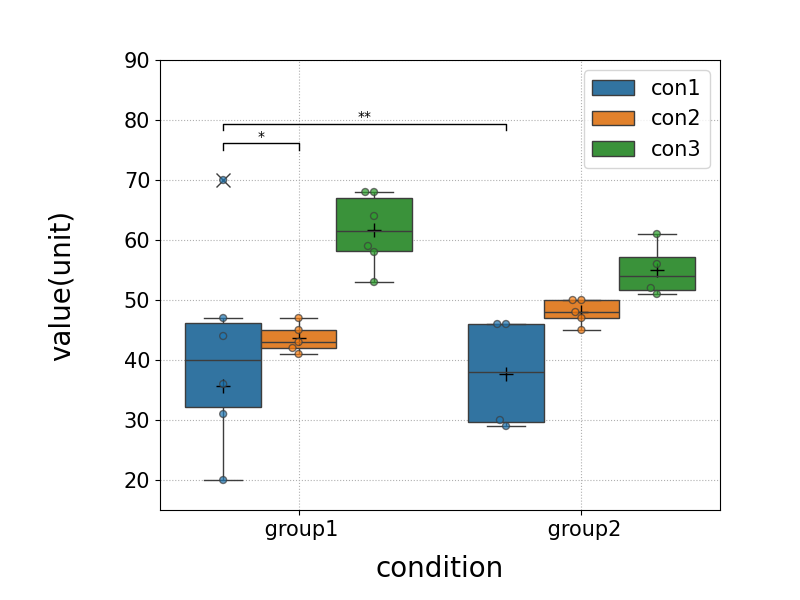
\includegraphics[width=0.6\textwidth]{figures/test/test.png}
    \caption{テスト画像の例}
    \label{fig:test_image_jp}
\end{figure}

画像パスはベストプラクティスに従い、プリアンブルの\texttt{\textbackslash graphicspath}設定により解決されます。

\section{参考文献の引用}

このセクションでは参考文献の引用例を示します。例として、Doe~\cite{example}による研究を参照します。

参考文献管理も.latexmkrcの設定により自動的に処理されます。

\section{まとめ}

本章では以下の要素を含むLaTeX文書作成のベストプラクティスを実装しました:

\begin{itemize}
    \item \texttt{graphicspath}による画像パス管理
    \item 相対パス参照による移植性の確保
    \item BibTeX参考文献管理
\end{itemize}
